\section{\secintegerdivision}
\label{sec_even_odd_divides}

In this section, we begin our exploration of integer division by discussing even and odd integers, divisors, and fractions.

 %%%%%%%%%%%%%%%%%%%%%%%%%%%%%%%%%%%%%%%

\newcommand{\sublockers}{Opening and Closing Lockers}
\subsection{\sublockers}
\label{sub_lockers}

But first, a puzzle.

\begin{act}[Lockers Puzzle]
\label{act_lockers}

    At Perpetual High School, a never-ending line of students marches down a never-ending hallway of lockers.  The first student opens each locker.  The second student closes every other locker (002, 004, 006, etc.) The third student changes the state of every third locker, which means closing 003, opening 006, etc.  And so on, with the $d^{th}$ student changing the state of every $d^{\text{th}}$ locker.

        \begin{figure}[hbtp]
            \centering
            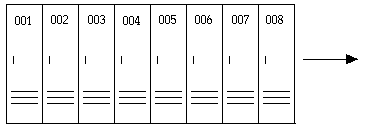
\includegraphics[scale=.8]{Puzzles/Puzzle_Images/Lockers.png}
            \caption{The first few lockers at Perpetual High School.}
            \label{fig_lockers}
        \end{figure}

    \begin{exerpart}
        \item Calculate the final state of each of the first ten lockers.  Show some work.
        \item How many students touch locker 100? Show work. 
        \item What is the final state of locker 100? Explain briefly.  
        \item \label{part_lockers} Make a conjecture about which lockers are finally left open and which are finally left closed. 
        \item There are two very reasonable answers to (\ref{part_lockers}).  One conjecture, Conjecture A, depends on the number of students who touch the locker. The other conjecture, Conjecture B, depends only on the locker number. Which conjecture did you make in (\ref{part_lockers}): A or B?  What is the other conjecture?
        \item Use whatever conjecture you prefer to determine whether locker \text{1,000,000} is open or closed.  Explain your reasoning.    
    \end{exerpart}
\end{act}

Be sure to complete \Cref{act_lockers} because we are about to reveal some of the answers.

\begin{exam}[Open lockers]
\label{exam_open_lockers}
~
    \begin{apart}
        \item What is the final state of locker 99?  Explain.
            \begin{soln}
                First note that the last student to touch locker 99 is the $99^{\text{th}}$ student.  So to determine the final state of locker 99 we only need to know which students from 1-99 touched it. We can factor 99 in several ways: $1 \times 99$, $3 \times 33$, and $9 \times 11$.  That is, the only students from 1-99 to touch locker 99 are students one, three, nine, 11, 33, and 99.  Student one opens locker 99, student three closes it, student nine opens it, student 11 closes it, student 33 opens it, and student 99 closes it.  The final state of locker 99 is that it is closed.
            \end{soln}
        \item Conjecture how the final state of a locker depends on the number of students who touch the locker.
            \begin{soln}
                When the number of students who touch the locker is even, as was the case for locker 99, the final state of the locker is closed.  When the number of students who touch the locker is odd, as was the case for locker 100, the final state of the locker is open.  This conjecture is Conjecture A.
            \end{soln}
        \item Conjecture which lockers have an odd number of students that touch that locker.
            \begin{soln}
                Notice that students who touch the locker tend to come in pairs.  For example, locker 99 is touched by students one and 99, students three and 33, and students nine and 11.  As another example, locker 100 is touched by students one and 100, students two and 50, students four and 25, and students five and 20.  But there is one additional student who touches locker 100, student 10, which makes the total number of students touching locker 100 odd.  Why is student 10 not in a pair?  Because $10 \times 10 = 100$ or, in other words, $100 = 10^2$.  We conjecture that lockers touched by an odd number of students have locker numbers equal to the square of an integer, known as a \vocab{perfect square}. This conjecture is Conjecture B.
            \end{soln}
    \end{apart}
\end{exam}

%%%%%%%%%%%%%%%%%%%%%%%%%%%%%%%%%%%%%%%

\newcommand{\subevenodd}{Even and Odd Integers}
\subsection{\subevenodd}
\label{sub_even_odd}

We have seen several situations in which it mattered whether an integer is even or odd.  An odd number of bridges was problematic in solving the Bridges Puzzle in \Cref{act_bridges}.  The chromatic number of the cycle $C_s$ and the wheels $W_s$ depended on whether $s$ was even or odd.  In each of those examples, we recognize that an even integer is the sum of twos: on-off, on-off, \ldots, on-off in the Bridges Puzzle or black-white, black-white, \ldots, black-white in coloring a cycle.  That is, $n$ is \vocab{even} if we can write 
    $$n = \underbrace{2 + 2 + 2 + \ldots + 2}_{k \text{ times}} = 2k.$$
Equivalently, we can think of even integers as those that divide exactly in half.  That is, $n=k+k = 2k.$  We state the formal definition. 

\begin{defn}[Even and odd]
\label{defn_even_odd}  
~
    \begin{apart}
        \item The integer $n$ is \vocab{even} if $n=2k$ for some integer $k$.  For example, 18 is even because $18=2(9)$. If we wanted to be formal, we would say $18=2k$ where $k=9$.
        \item The integer $n$ is \vocab{odd} if $n=2k+1$ for some integer $k$.  For example, 19 is odd because $19 = 2(9)+1$. If we wanted to be formal, we would say $19=2k+1$ where $k=9$.
    \end{apart}
\end{defn}

Here are some more general examples.

\begin{exam}[Even and odd, in general]
\label{exam_even_odd_general} 
You probably know many facts about even and odd integers.  In this example, we use only the definitions. 
    \begin{apart}
        \item Use the definition of even to show that $6t$ is even for any integer $t$.
            \begin{soln}
                We want to write $6t=2k$ for some integer $k$.  We can solve to find $k$. We divide by two to get $k=3t$, which is an integer. Officially, we need to use that value of $k$ to write $$6t=2(3t),$$ so $6t$ is even. 
                
                Notice that we could have just factored out the two to write $$6t=2(3t)$$ without any mention of $k$.
            \end{soln}
        \item Use the definition of odd to show that $2m-1$ is odd for any integer $m$.
            \begin{soln}
                We want to write $2m-1 = 2k+1$ for some integer $k$.  We can solve to find $k$.  First, we subtract and factor to get $2k=(2m-1)-1=2m-2=2(m-1)$. Next, we divide by two to get $k=m-1$, which is an integer. Officially, we need to use that value of $k$ to write $$2m-1= 2(m-1)+1,$$ so $2m-1$ is odd.

                Notice that we could have used algebra to write $$2m-1 = 2m-2+1 = 2(m-1) + 1$$ without any mention of $k$.
            \end{soln}
    \end{apart}
\end{exam}

Try working with these definitions.  As before, you should not use facts that you might know about even and odd integers.

\begin{act}[Even and odd]
\label{act_even_odd}
~ 
    \begin{actpart}
        \item Use the definition of even to show that 34 is even.
        \item Use the definition of odd to show that 37 is odd. 
        \item \label{part_0is_even} Is zero even, odd, both, or neither? Justify your answer.
        \item Give examples of integers $m$ to show that $3m+1$ can be even or odd.  
        \item Use the definition of odd to show that, for any integer $m$, the integer $4m+1$ is always odd.  Hint: Once you find a useful value of $k$, write $4m+1$ in the form $2k+1$.
    \end{actpart}  
\end{act}

In \Cref{act_even_odd} (\ref{part_0is_even}) we asked if zero is even, odd, both, or neither.  A common incorrect answer is neither, perhaps because neither is the correct answer to a different question, namely is zero positive, negative, both, or neither?  Let's show that zero is even and not odd.

\begin{exam}[Zero is even]
\label{exam_0is_even}
~
    \begin{apart}
        \item Use the definition to show that zero is even.
            \begin{soln}
                We can write $0 = 2(0)$.  That is $0 = 2k$ when $k=0$.  Since $k=0$ is an integer, it follows that zero is even.
            \end{soln}
        \item Use the definition to show that zero is not odd.
            \begin{soln}
                Suppose that we could write $0 = 2k+1$.  We can subtract one to get $2k=-1$ and then divide by two to get $k = ^-\frac{1}{2}$.  Since $^-\frac{1}{2}$ is the only possible value of $k$, and $^-\frac{1}{2}$ is not an integer, it follows that zero is not odd.
            \end{soln}
    \end{apart}
\end{exam}

It turns out that every integer is even or odd and never both.  We prove this result in \Cref{exam_every_integer_even_or_odd}.

%%%%%%%%%%%%%%%%%%%%%%%%%%%%%%%%%%%%%%%
\newcommand{\subdivides}{Divisibility}
\subsection{\subdivides}
\label{sub_divides}

In the Lockers Puzzle (\Cref{act_lockers}), the $d^{\text{th}}$ student touches locker $d$, locker $d+d=2d$, locker $d+d+d=3d$, etc.  In general, the $d^{\text{th}}$ student touches locker $n$ when we can write $$n=\underbrace{d+d+ \ldots+d}_{k \text{ times}} =dk$$ for some integer $k$.  We make this concept formal with another definition.

\begin{defn}[Divides]
\label{defn_divides}
~
    \begin{apart}
        \item The nonzero integer $d$ \vocab{divides} integer $n$, denoted $d \mid n$, if $n = dk$ for some integer $k$.  For example, 3 divides 15, denoted $3 \mid 15$ because $15 = 3(5)$.  Note also that $3 \mid -15$ because $-15 = 3(-5)$ and $-3 \mid 15$ because $15 = -3(-5)$.
        
        \item If $d \mid n$, then $d$ is a \vocab{divisor}  (or \vocab{factor}) of $n$.  For example, the (positive) divisors of 15 are: 1, 3, 5, and 15 because $1 \times 15 = 15$ and $3 \times 5=15$. (It is harder to know that we found all the positive divisors.) The complete list of 15 divisors is $\pm$ 1, $\pm$ 3, $\pm$ 5 and $\pm$ 15.
        
        \item If $d \mid n$, then $n$ is a \vocab{multiple} of $d$.  For example, 10, -35, and 65 are multiples of 5.
        
        \item If $d$ does not divide $n$, we write $d \nmid n$.  For example, $4 \nmid 15$.
    \end{apart}
\end{defn}

Here are some more general examples.

\begin{exam}[Divides, in general]
\label{exam_divides_general}
    You might know many facts about divisibility. In this example, we use only the definition.
    \begin{apart}
        \item \label{part_65mult5} Show that 65 is a multiple of 5.
        \begin{soln}
            Note that $5 \times 13 = 65$ and so $65 = 5(13)$.  Thus, 65 is a multiple of 5.  
        \end{soln}
        \item Rewrite the statement from (\ref{part_65mult5}) using the word ``divides'' and divides notation.
        \begin{soln}
            We say that 5 divides 65, denoted $5 \mid 65$.
        \end{soln}  
        \item Use the definition of divides to show that $5 \mid (5n-20)$.
        \begin{soln}
            Factor to write $5n-20 = 5(n-4)$, so $5 \mid (5n-20)$. If we wanted to be formal, we could write $5n-20 = 5k$ where $k=n-4$.
        \end{soln}
    \end{apart}
\end{exam}

It is your turn to practice with divides.

\begin{act}[Divides]
\label{act_divides}
~
    \begin{actpart}
        \item List the divisors of 12.  Note: do not forget the negative divisors.
        \item Give an example of three different integers that are multiples of 12.
        \item Which is true: $12 \mid 6$ or $6 \mid 12$?  Justify your answer.
        \item Use the definition of divides to show that $10 \mid (100k-30)$.
        \item Use the definition of divides to show that $1 \mid n$ for all integers $n$.        
        \item  \label{part_does_0dividen} Is $0 \mid n$ true for all nonzero integers $n$?  Justify your answer.
        \item \label{part_does_ndivide0} Is $n \mid 0$ true for all nonzero integers $n$?  Again, justify your answer.
    \end{actpart}
\end{act}

You may have heard, correctly, that we cannot divide by zero.  Let's take a closer look at \Cref{act_divides} (\ref{part_does_0dividen}) and (\ref{part_does_ndivide0}).

\begin{exam}[You cannot divide by zero]
\label{exam_cannot_divide_by0}
~
    \begin{apart}
        \item  Can we divide by zero?  That is, is zero a divisor of any integer?  Explain.
            \begin{soln}
                We are asking if $0 \mid n$ for any integer $n$. In \Cref{defn_divides}  we did not allow the divisor $d$ to be zero, so the answer is no.  The reason we excluded zero is because if $n = 0(k) =0$ for some integer $k$, then the only possibility is $n=0$.  Therefore, it is impossible for zero to divide any nonzero integer. We also do not allow zero to divide itself either.  The answer is no.
            \end{soln}
        \item Is zero a multiple of any integer?
            \begin{soln}
                We are asking if $n \mid 0$ for any integer $n$.  That means we are looking for an integer $k$ such that $0 = (n)k$.  Since $0 = (n)0$ and $k=0$ is an integer, it follows that $n \mid 0$ for all nonzero integers $n$. The answer is yes.
            \end{soln} 
    \end{apart}
\end{exam}

%%%%%%%%%%%%%%%%%%%%%%%%%%%%%%%%%%%%%%%
\newcommand{\subfractions}{Algebra: Equivalent Fractions}
\subsection{\subfractions}
\label{sub_fractions}

When we divide one integer by another (nonzero) integer, sometimes we get an integer, but sometimes we get a fraction (rational number) that is not an integer.  Here is the formal definition.

\begin{defn}[Fraction (rational number)]
\label{defn_fraction_rational}   
~
    \begin{apart}
        \item For integer $n$ and nonzero integer $d$, the \vocab{fraction} (or \vocab{rational number}) is the number we get by dividing $n$ by $d$, meaning
        $$\displaystyle \frac{n}{d} = n \div d.$$  
        We can think of the fraction $\frac{n}{d}$ as representing an equal share of $n$ objects among $d$ places.  For example, if we have 40 cucumber slices and five pickling jars, then we can put $40 \div 5 = 8$ slices in each jar.  Similarly, if we have four party-sized bags of candy to share equally among ten people, then each person gets $\frac{4}{10} = 4 \div 10 = .4 = 40\%$ of a bag.
        \item Note that any integer is a fraction because $$\frac{n}{1} = n \div 1 = n.$$  For example, $ 4 = \frac{4}{1}.$
        
        \item In the fraction $\frac{n}{d},$ the integer on the top of the fraction $n$ is the \vocab{numerator} and the integer on the bottom of the fraction $d$ is the \vocab{denominator}. For example, in the fraction $\frac{4}{10}$ the numerator is four and the denominator is ten.
        
        \item \label{part_defn_equal_fractions} For integers $n$, $m$, $a \neq 0$, and $b \neq 0$, the fractions
        $\frac{n}{a}$ and 
        $\frac{m}{b}$ are \vocab{equal} (or \vocab{equivalent}), which we write as
        $$\frac{n}{a}=\frac{m}{b},$$ if $nb=ma.$
        For example, $\frac{6}{15} = .4$ and so      
        $\frac{4}{10}=\frac{6}{15}.$
        We can \vocab{cross-multiply} to confirm that $(4)(15) = 60 = (6)(10).$        
    \end{apart}
\end{defn}

There is a connection between divides and fractions.

\begin{rem} [Fractions and divisibility]
\label{rem_fractions_divides}
    Let $d$ and $n$ be integers with $d\neq 0$. Then $d \mid n$ exactly when $\frac{n}{d}$ is an integer.  Although we have this connection between fractions and divisibility, it is customary to avoid referencing fractions when working with divides.
\end{rem}

Every fraction has (infinitely) many different names.  We often want to write a fraction in its simplest form. Other times, it is useful to write a fraction with a denominator such that the fraction is not in its simplest form-- for example, to add, subtract, or compare fractions.  The next theorem verifies both operations.

\begin{thm}[Equal fractions]
\label{thm_equal_fractions}
    For integer $n$ and nonzero integers $d$ and $c$,    
    \begin{apart}
        \item \label{part_thm_common_denom} If we multiply the numerator and denominator of a fraction by a nonzero integer, the resulting fraction is equal to the original fraction, namely
        $$\frac{n}{d} =  \frac{c(n)}{c(d)}.$$ 

        \item \label{part_thm_reduce_fraction} This equation holds in both directions.  Specifically, we can \vocab{cancel a common nonzero factor} (or \vocab{reduce} the fraction) using the equation 
        $$\frac{c(n)}{c(d)}= \frac{n}{d}.$$
    \end{apart}     

    \begin{proof} Let $n$, $d$, and $c \neq 0$ be integers.  By the commutative and associative properties,
        $$
        n(c(d)) 
        = n \times c \times d 
        = c \times n \times d
        = (c(n))d
        $$
    and so, by \Cref{defn_fraction_rational} (\ref{part_defn_equal_fractions}), 
    $$\frac{n}{d} =  \frac{c(n)}{c(d)},$$ as in (\ref{part_thm_common_denom}).  Note that (\ref{part_thm_reduce_fraction}) is the same equation read right-to-left instead.      
    \end{proof}
\end{thm}

Let's see this theorem in action.

\begin{exam}[Equal fractions]
\label{exam_equal_fractions}
~
    \begin{apart}
        \item \label{part_twofifths} Write $\frac{2}{5}$ as a fraction with denominator 15.
        \begin{soln}
            Since $15=3 \times 5$, we can use \Cref{thm_equal_fractions} to multiply top and bottom of the fraction by three to get
            $$\frac{2}{5} =\frac{3(2)}{3(5)}
            =\frac{6}{15}.$$
        \end{soln}

        \item Which fraction is larger: $\frac{2}{5}$ or $\frac{1}{3}$?
        \begin{soln}
            We can write each fraction with \vocab{common denominator} $3 \times 5 = 15.$  In part (\ref{part_twofifths}), we found $\frac{2}{5} =\frac{6}{15}.$ Similarly, we can use \Cref{thm_equal_fractions} to multiply top and bottom of the fraction $\frac{1}{3}$ by five to get:
            $$\frac{1}{3} =\frac{5(1)}{5(3)}
            =\frac{5}{15}.$$
            We can imagine $\frac{6}{15}$ as the amount of pizza each person gets if we have six pizzas shared by 15 people.  In that vein, we can imagine $\frac{5}{15}$ as the amount of pizza each person gets if we have five pizzas shared by 15 people. Each person will get more pizza if we have six pizzas to share versus five pizzas to share, and so $\frac{6}{15}> \frac{5}{15}$.
            It follows that $\frac{2}{5}>\frac{1}{3}.$
        \end{soln}

        \item Reduce the fraction $\frac{24}{100}$.
        \begin{soln}
            Notice that $4 \mid 24$ and $4 \mid 100$.  By \Cref{thm_equal_fractions} we have
            $$\frac{24}{100} = \frac{4(6)}{4(25)}= \frac{6}{25}.$$
            Notice that 6 and 25 do not have any common divisors (other than the integers $\pm$1) and so we cannot further reduce the fraction $\frac{6}{25}$.
        \end{soln}
    \end{apart}
\end{exam}

The concept of a fraction that cannot be further reduced has a formal name.

\begin{defn}[Lowest terms]
\label{defn_lowest_terms}
~
    \begin{apart}
        \item The integers $s$ and $t$ are \vocab{coprime} (or \vocab{relatively prime}) if the only common positive divisor of $s$ and $t$ is the integer 1.  For example, 6 has positive divisors 1, 2, 3, and 6 whereas 25 has positive divisors 1, 5, and 25 so their only common positive divisor is 1.  Therefore, 6 and 25 are coprime.
        \item The fraction $\frac{s}{t}$ is \vocab{written in lowest terms} if $s$ and $t$ are coprime. For example, since 6 and 25 are coprime, it follows that the fraction $\frac{6}{25}$ is written in lowest tersm.
    \end{apart}
\end{defn}

We revisit the concept of coprime in \Cref{sec_gcd}.  Let's practice reducing fractions.

\begin{act}[Equivalent fractions]
\label{act_equiv_fractions}
~
    \begin{apart}
        \item Reduce $\displaystyle \frac{15}{70}$ to lowest terms.
        \item Reduce $\displaystyle\frac{5!}{6!}$ to lowest terms. 
        
        Hint: Use the definition of factorial (\Cref{defn_factorial}) and cancel before multiplying.
        \item Reduce $\displaystyle\frac{98!}{100!}$ to lowest terms.
        \item Write the product $(10)(9)(8)(7)$ as a fraction whose numerator and denominator are each a single factorial.        
        \item Reduce $\displaystyle\frac{2^3}{2^5}$ to lowest terms. 
        
        Hint: Use the definition of exponential notation (\Cref{defn_exp_notation}) and cancel before multiplying.              
        \item Reduce $\displaystyle\frac{2^{40}}{2^{100}}$ to lowest terms.
        \item Write as a single power of 10:
        $\displaystyle\frac{10^n}{10}.$
        \item Write as a single power of 10:
        $\displaystyle\frac{10^n}{100}.$
        Hint: $100 = 10 \times 10$.
    \end{apart}
\end{act}

We look at a few examples similar to \Cref{act_fractions}.

\begin{exam}[Equivalent fractions]
\label{exam_equiv_fractions}
~
    \begin{apart}
        \item Reduce $\displaystyle\frac{48!}{50!}$ to lowest terms.
            \begin{soln}
                Let's use the definition of factorial and cancel before multiplying to get
                    $$\frac{48!}{50!} 
                    = \frac{(48)(47)\cdots(3)(2)(1)}{(50)(49)(48)(47)\cdots(3)(2)(1)}
                    = \frac{48!}{(50)(49)(48!)}
                    = \frac{1}{(50)(49)}.$$
                Note that we cancel the common factor of $c=48!=(48)(47)\cdots(3)(2)(1)$.
            \end{soln}
        \item \label{part_3string_letters} How many strings of three uppercase letters are there if we cannot repeat letters?
            \begin{soln}
                Think of filling in three spaces with uppercase letters. The first space can be any of the 26 uppercase letters. Because repeats are not allowed, the second space can be any of the 25 remaining uppercase letters, and the third space can be any of the 24 remaining uppercase letters.  Since steps multiply (\Cref{thm_steps_multiply}), the answer is $(26)(25)(24)$.
            \end{soln}
        \item Write your answer to (\ref{part_3string_letters}) as a fraction whose numerator and denominator are each a single factorial.                     
            \begin{soln}
                Notice that $(26)(25)(24)$ looks like the beginning of 26!  We can multiply the numerator and denominator by $c=23!$ to get
                    $$(26)(25)(24)= \frac{(26)(25)(24)}{1}
                    = \frac{(26)(25)(24)(23!)}{23!}
                    = \frac{(26)(25)(24)(23)(22) \cdots (3)(2)(1)}{(23)(22) \cdots (3)(2)(1)}
                    = \frac{26!}{23!}$$
            \end{soln}
        \item Reduce $\displaystyle\frac{10^{20}}{10^{35}}$ to lowest terms.
            \begin{soln}
                Let's use the definition of exponential notation and cancel before multiplying to get
                    $$\frac{10^{20}}{10^{35}}
                    = \frac{\overbrace{10 \times 10 \times \ldots \times 10}^{20 \text{ times}}}{\underbrace{10 \times 10 \times \ldots \times 10}_{35 \text{ times}}}
                    = \frac{1}{\underbrace{10 \times 10 \times \ldots \times 10}_{15 \text{ times}}} 
                    = \frac{1}{10^{15}}.
                    $$
                Note that we canceled 20 factors of 10 to get $35-20=15$ remaining factors of 10.
            \end{soln}
        \item Write as a single power of 2:
        $\displaystyle\frac{2^n}{2}.$
            \begin{soln}
                Let's use the definition of exponential notation and cancel before multiplying to get
                    $$\frac{2^n}{2}
                    = \frac{\overbrace{2 \times 2 \times \ldots \times 2}^{n \text{ times}}}{2}
                    = \frac{\overbrace{2 \times 2 \times \ldots \times 2}^{n-1 \text{ times}}}{1}
                    = 2^{n-1}
                    $$
                Note that we canceled one of the $n$ factors of two to get $n-1$ remaining factors of two.
            \end{soln}
    \end{apart}
\end{exam}

%%%%%%%%%%%%%%%%%%%%%%%%

\subsection{Exercises}

%%%%%%%%%%%%%%%%%%%%%%%%

\subsubsection{Exercises for \Cref{sub_lockers} \sublockers}

\begin{exer}[\exerP] % final state locker 24]
\label{exer_locker24}  
Without using any conjectures from \Cref{act_lockers}, explain how to find the final state of Locker 24.  Be detailed.
\end{exer}

\begin{exer}[\exerU] % lockers touched two or three times]
\label{exer_lockers_2or3}
~
    \begin{exerpart}
        \item In the Lockers puzzle (\Cref{act_lockers}), Locker 001 is only touched once.  Of all the lockers, which are only touched twice? Make a conjecture that depends on only the locker number.
        \item Which lockers are touched exactly three times? Make a conjecture that depends on only the locker number.    
    \end{exerpart}  
\end{exer}

%\begin{exer}[\exerR] % Opening and Closing Lockers
% \label{exer_dyk_lockers}
%     Do you know \ldots
%         \begin{exerpart}
%             \item 
%         \end{exerpart}
% \end{exer}

\begin{exer}[\exerE] % lockers touched most]
\label{exer_lockers_touchedmost}
~
    \begin{apart}
        \item Of the first 50 lockers, which are touched by the most students in the Lockers Puzzle (\Cref{act_lockers})?  Do not use technology or other resources to find the answer.  Show work. 
        \item Of the first 1,000 lockers, which are touched by the most students in the Lockers puzzle (\Cref{act_lockers})?  Use technology or other resources to find the answer.  Explain what you looked up and cite your source(s). 
    \end{apart}      
\end{exer}

%%%%%%%%%%%%%%%%%%%%%%%%

\subsubsection*{Exercises for \Cref{sub_even_odd} \subevenodd}

When an exercise asks you to use the definition of even or odd, you should use only that definition and algebra.  Do not use other facts you might know about even or odd integers.

\begin{exer}[\exerP] % 2026 is even, 2025 is odd]
\label{exer_2026even_2025odd}
~
    \begin{exerpart}
        \item Use the definition of even to show that 2026 is even.
        \item Use the definition of odd to show that 2025 is odd.       
    \end{exerpart}
\end{exer}

\begin{exer}[\exerP] % examples of even and odd sums and products]
\label{exer_examples_even_odd_sum_product}
~
    \begin{exerpart}
        \item Give an example of two integers whose sum is even and whose product is odd.
        \item Give an example of two integers whose sum is odd and whose product is even.
        \item Is it possible to have two integers whose sum and product are both even?  If so, give an example.
        \item Is it possible to have two integers whose sum and product are both odd?  If so, give an example.
    \end{exerpart}
\end{exer}

\begin{exer}[\exerU] % linear expressions even or odd.]
\label{exer_linears_even_odd}
~  
    \begin{exerpart}
        \item \label{part_6qminus10_is_even} For any integer $q$, use the definition of even to show that $6q-10$ is even. 
        \item For any integer $m$, use the definition of odd to show that $4m+7$ is odd. %$\triangleright$ The symbol $\triangleright$ indicates that a video solution is available.
        \item Give examples of integers $m$ to show that $5m+1$ can be even or odd.  
    \end{exerpart}
\end{exer}

\begin{exer}[\exerR] % Even and Odd Integers
\label{exer_dyk_even_odd}
    Do you know \ldots
        \begin{exerpart}
            \item How even and odd are defined?
            \item How to use the definition to show that an integer is even or odd?
        \end{exerpart}
\end{exer}

\begin{exer}[\exerE] % evens and odds alternate]
\label{exer_prove_consecutive_even_odd}  
~
    \begin{exerpart}
        \item Consider an even integer $n$.  Use the definitions of even and odd to show that the next consecutive integer, $n+1$, is odd.
        \item Consider an odd integer $n$.  Use the definitions of even and odd to show that the next consecutive integer, $n+1$, is even.
    \end{exerpart}
\end{exer}

%%%%%%%%%%%%%%%%%%%%%%%%

\subsubsection*{Exercises for \Cref{sub_divides} \subdivides}

When an exercise asks you to use the definition of divides, you should use only that definition and algebra.  Do not use other facts you might know about divisibility. 

\begin{exer}[\exerP] % divides notation]
\label{exer_divides_notation}
~
    Rewrite each statement using the divides symbol $\mid$ or $\nmid$.
    \begin{exerpart}
        \item 15 divides 105
        \item 56 is a multiple of seven
        \item 56 is not a multiple of 11
        \item 44 is a divisor of 44
        \item one is a divisor of 44
        \item 50 is even
        \item 51 is odd
    \end{exerpart}   
\end{exer}

\begin{exer}[\exerP] % list divisors]
\label{exer_list_divisors}
    List all the positive divisors of each integer.  Do not use technology or other resources.
        \begin{exerpart}
            \item seven
            \item 10
            \item 80
            \item 81
        \end{exerpart}
\end{exer}

\begin{exer}[\exerU] % applying divides]
\label{exer_prove_divides}  
A teacher has a class of 20 students, and he wants to arrange them into equally sized groups.  
    \begin{exerpart}
        \item Use the definition of divides to show that $4 \mid 20$. 
        \item Could the teacher divide the students into equally sized groups of size four?  How many groups would there be? Explain. 
        \item Use the definition of divides to explain why groups of size three would not work. 
        \item \label{part_divisors20} What size groups could the teacher use?  Explain. 
        \item How would your answer to (\ref{part_divisors20}) change if two students are absent? 
    \end{exerpart}
\end{exer}

\begin{exer}[\exerU] % show divisor or multiple]
\label{exer_prove_divides_general}  
~
    \begin{exerpart}
        \item Use the definition of divides to show that four is a divisor of $4q-8$ for any integer $q$. 
        \item Use the definition of divides to show that $14m$ is a multiple of 7, for any integer $m$.
    \end{exerpart}
\end{exer}

\begin{exer}[\exerU] % divides $n$]
\label{exer_dividesn}
~
    \begin{exerpart}
        \item Use the definition of divides to show that $n \mid n$ for any integer $n$.  
        \item Is it possible to have positive integers $b$ and $n$ with $b \mid n$ and $n \mid b$?  Explain.
    \end{exerpart}
\end{exer}

\begin{exer}[\exerU] %divisors of factorials]
\label{exer_divisors_of_factorials}
    Factorials were defined in \Cref{defn_factorial}.  In this problem, do not use technology or other resources.
        \begin{exerpart}
            \item Show that $7 \mid 9!$ 
            \item Show that $7! \mid 9!$
            \item Show that $10 \mid 9!$
        \end{exerpart}
\end{exer}

\begin{exer}[\exerR] % Divisibility
\label{exer_dyk_divides}
    Do you know \ldots
        \begin{exerpart}
            \item What $d \mid n$ and $d \nmid n$ mean?
            \item How to show that $d \mid n$?
            \item How to write statements about divisors or multiples using $\mid$?
            \item How to find divisors or multiples of an integer? 
        \end{exerpart}
\end{exer}

\begin{exer}[\exerE] % divides a square]
\label{exer_divides_square}  
~
    \begin{exerpart}
        \item Consider an integer $n$ such that $4 \mid n$.  Use the definition of divides to show that $4 \mid n^2$.
        \item Give an example of an integer $m$ such that $4 \mid m^2$ but $4 \nmid m$.
    \end{exerpart}
\end{exer}

%%%%%%%%%%%%%%%%%%%%%%%%

\subsubsection*{Exercises for \Cref{sub_fractions} \subfractions}

\begin{exer} [\exerP] % equal fractions]
\label{exer_equal_fractions}
~
    \begin{exerpart}
        \item Write $\frac{7}{10}$ as a fraction with denominator 30.
        \item Which fraction is larger: $\frac{7}{10}$ or $\frac{2}{3}$?  Use a common denominator to compare the fractions.
        \item List the positive divisors of nine and ten to show that 9 and 10 are coprime.
        \item Reduce the fraction $\frac{450}{500}$ to lowest terms.
    \end{exerpart}
\end{exer}

\begin{exer} [\exerU] % reduce fractions with factorials]
\label{exer_reduce_fraction_factorials}
~
    \begin{exerpart}
        \item Reduce $\displaystyle \frac{6!}{8!}$ to lowest terms.
        
        Hint: Use the definition of factorial (\Cref{defn_factorial}) and cancel before multiplying.
        \item Write the product $(5)(4)(3)$ as a fraction whose numerator and denominator are each a single factorial.
         \item Reduce $\displaystyle \frac{10!}{2!8!}$ to lowest terms.
        \item \label{part_nchoose2_formula} Conjecture how to write $\displaystyle \frac{n!}{2!(n-2)!}$ in lowest terms.
        \item Where have you seen the answer to (\ref{part_nchoose2_formula}) before?
    \end{exerpart}
\end{exer}

\begin{exer}[\exerR] % Algebra: Fractions
\label{exer_dyk_fractions}
    Do you know \ldots
        \begin{exerpart}
            \item How a fraction is related to integer division?
            \item What the numerator and denominator of a fraction are?
            \item How to write a fraction over a new denominator?
            \item How to reduce a fraction to lowest terms?
            \item What it means to say that two integers are coprime?
        \end{exerpart}
\end{exer}

\begin{exer} [\exerE] % reduce fractions with powers]
\label{exer_reduce_fractions_powers}
    For this exercise, all exponents should be nonnegative. (If you have seen negative exponents, the answers should still make sense, just use nonnegative exponents.)
    \begin{exerpart}
        \item Reduce $\displaystyle \frac{2^{11}}{2^5}$ to lowest terms.
        
        Hint: Use the definition of exponential notation (\Cref{defn_exp_notation}) and cancel before multiplying.
        \item Reduce $\displaystyle \frac{2^5}{2^{11}}$ to lowest terms.
        \item Conjecture how to write $\displaystyle \frac{2^a}{2^b}$ in lowest terms when $a<b$ and when $a >b$.  What happens when $a=b$?
    \end{exerpart}
\end{exer}

%%%%%%%%%%%%%%%%%%%%%%%%%%%
\subsection{\answers}
%%%%%%%%%%%%%%%%%%%%%%%%%%%

%%%%%%%%%%%%%%%%%%%%%%%%%%
\subsubsection{\answers for \Cref{sub_lockers} \sublockers}

\subsubsection*{\Cref{exer_locker24} \answers}
   Hint: It is closed.
   
\subsubsection*{\Cref{exer_lockers_2or3} \answers}
\begin{apart}
    \item Hint: Examples include lockers 2, 3, 5, 7, 11.
    \item Hint: They are open.
\end{apart}

%%%%%%%%%%%%%%%%%%%%%%%%%%
\subsubsection{\answers for \Cref{sub_even_odd} \subevenodd}

\subsubsection*{\Cref{exer_2026even_2025odd} \answers}
\begin{apart}
    \item Hint: Write $2026 = 2(\hspace{0.5in})$ and fill in the parentheses.
    \item Hint: Write $2025 = 2(\hspace{0.5in})+1$ and fill in the parentheses.
\end{apart}

\subsubsection*{\Cref{exer_examples_even_odd_sum_product} \answers}
\begin{apart}
    \item Hint: Both integers must be odd.
    \item Hint: One integer must be odd and the other integer must be even.
    \item Hint: Yes, both integers must be even.
    \item No
\end{apart}

\subsubsection*{\Cref{exer_linears_even_odd} \answers}
\begin{apart}
    \item Hint: Write $6q-10=2(\hspace{0.5in})$ and fill in the parentheses.
    \item Hint: Write $4m+7=2(\hspace{0.5in})+1$ and fill in the parentheses.If you need help figuring out what goes into the parentheses, solve $4m+7=2k+1$ for $k$.  
    \item Hint:  One example should use an even value of $m$ and the other example should use an odd value of $m$.
\end{apart}

\subsubsection*{\Cref{exer_prove_consecutive_even_odd} \answers}
\begin{apart}
    \item Hint: Write $n=2k$ and then evaluate $n+1$.
    \item Hint: Write $n=2k+1$, simplify $n+1$, and then factor out two.
\end{apart}

%%%%%%%%%%%%%%%%%%%%%%%%%%

\subsubsection{\answers for \Cref{sub_divides} \subdivides}

\subsubsection*{\Cref{exer_divides_notation} \answers}
\begin{apart}
    \item $5 \mid 105$
    \item Hint: If $a \mid b$, then the integer $a$ is smaller than (or equal to) the integer $b$.
    \item Hint: The answer uses $\nmid$.
    \item $44 \mid 44$
    \item Hint: If $a \mid b$, then the integer $a$ is smaller than (or equal to) the integer $b$.
    \item Hint: The answer involves the integer two.
    \item Hint: The answer involves the integer two.
\end{apart}

\subsubsection*{\Cref{exer_prove_divides} \answers}
\begin{apart}
    \item Hint: Write $4q-8=4(\hspace{0.5in})$ and fill in the parentheses.
    \item Hint: Write $14m=7(\hspace{0.5in})$ and fill in the parentheses.
\end{apart}

\subsubsection*{\Cref{exer_divisors_of_factorials} \answers}
\begin{apart}
    \item Hint: Write $9!=7(\hspace{0.5in})$ and fill in the parentheses with the product of the other factors of $9!$
    \item Hint: Write $9!=7!(\hspace{0.5in})$ and fill in the parentheses with the product of the other factors of $9!$
    \item Hint: Use $10=(5)(2)$. Write $9!=10(\hspace{0.5in})$ and fill in the parentheses with the product of the other factors of $9!$
\end{apart}

\subsubsection*{\Cref{exer_divides_square} \answers}
\begin{apart}
    \item Hint: Write $n=4k$, expand and simplify $n^2$, and then factor out four.
    \item Hint: The integer $m$ must be even.
\end{apart}

%%%%%%%%%%%%%%%%%%%%%%%%%%

\subsubsection{\answers for \Cref{sub_fractions} \subfractions}

\subsubsection*{\Cref{exer_equal_fractions} \answers}
\begin{apart}
    \item $\frac{21}{30}$
    \item Hint: $\frac{2}{3}=\frac{20}{30}$
    \item Hint: The positive divisors of nine are one, three, and nine.  What are the positive divisors of 10?
    \item Hint: Use \Cref{thm_equal_fractions} (\ref{part_thm_reduce_fraction}) with $c=5$.
\end{apart}

\subsubsection*{\Cref{exer_reduce_fraction_factorials} \answers}
\begin{apart}
    \item $\frac{1}{56}$
    \item $\frac{5!}{2!}$
    \item 45 (or $\frac{45}{1}$)
    \item Hint: $n!=(n)(n-1)\underbrace{(n-2)\cdots(3)(2)(1)}_{(n-2)!}$
    \item Handshakes puzzle (or $\binom{n}{2}$)
\end{apart}

\subsubsection*{\Cref{exer_reduce_fractions_powers} \answers}
\begin{apart}
    \item $2^6$ (or $\frac{2^6}{1})$
    \item $\frac{1}{2^6}$
    \item Hint: When $a < b$, we have $\frac{2^a}{2^b} = \frac{1}{2^{b-a}}$. 
\end{apart}